\documentclass{article}
\usepackage[a4paper,margin=2.8cm]{geometry}

\usepackage{lmodern}
\usepackage[french]{babel}
%\usepackage{fourier}
\usepackage[utf8]{inputenc}
\usepackage[T1]{fontenc}
\usepackage{mathtools, amssymb,amsthm}


\usepackage{url,mdframed}
\usepackage{hyperref}

\def\separateur{\begin{center}
$\star$\\
$\star\quad\star$
\end{center}}

\begin{document}
\author{Damien Mégy}
\title{Bibliographie commentée\\Troisième année de Licence de mathématiques \\ \&\\ Première année de Magistère de mathématiques}

\maketitle
\tableofcontents

\section*{Comment utiliser cette bibliographie}
\begin{itemize}
\item Les sous-sections correspondent plus ou moins aux UE de la L3.
\item À chaque fois, la ou les premières première référence sont encadrées et  particulièrement recommandées. Souvent, il s'agit de références incontournables, plébiscitées par des générations successives d'étudiants et collègues. 
\item La liste contient des ouvrages d'autrices ou auteurs étrangers. Il est  extrêmement enrichissant de les lire ou au moins de les parcourir afin de réaliser la variété de points de vue existants.
\item Les livres sont de différentes sortes : certains sont juste de bons supports de révisions, d'autres vous apprendront vraiment des mathématiques. À trier suivant les besoins du moment.
\item La liste est (trop) longue. Lire quelques livres cités ici (ou d'autres) est déjà très bien, même juste deux ou trois. Par contre, ne lire \emph{aucun} livre de mathématiques pendant son année de L3 serait dommage voire considéré comme un peu anormal. 
\end{itemize}

\section*{Comment ne pas utiliser cette bibliographie}
\begin{itemize}
\item Lire les livres dans l'ordre de la liste, en commençant par le début.
\item Commencer par la fin, par les ouvrages avancés, et être dégoûté.
\item Ne lire aucun livre.
\item Ne pas lire la liste du tout.
\end{itemize}

\newpage
\section{Bibliographie pour la L3}

\subsection{Fondements, redécouverte du programme de L1-L2 ou CPGE}
\begin{mdframed}
\begin{itemize}
\item Richard Courant, Herbert Robbins, \emph{Qu'est-ce que les mathématiques ?}
\begin{quote}
Enfin traduit en français, par Marie Anglade et Karin Py. En discutant entre collègues (français mais surtout internationaux), on constate que beaucoup ont été marqués par ce livre dans leur jeunesse. D'une richesse exceptionnelle, l'ouvrage démarre au niveau bac+1 mais contient de nombreux thèmes de  niveau bac+3.% https://images.math.cnrs.fr/billets/le-courant-et-robbins/
\end{quote}
\item Bertrand Hauchecorne, \emph{Les contre-exemples en mathématiques}
\begin{quote}
522 contre-exemples couvrant la plupart des chapitres des deux premières années. (Manque un peu de contre-exemples en probabilités.)
\end{quote}
\end{itemize}
\end{mdframed}
\begin{itemize}
%\item A. Rajwade, A. Bhandari, \emph{Surprises and Counterexamples in Real Function Theory}
%\begin{quote}
%Plus qu'une liste de contre-exemples, ce livre s'attarde sur certains objets étonnants de l'analyse réelle. 
%\end{quote}
\item Walter Rudin, \emph{Principes d'analyse mathématique}
\begin{quote}
Traduit de l'anglais par Guy Auliac. Surnommé le \og baby Rudin\fg{} par les anglo-saxons, cet excellent ouvrage prend l'analyse à son début, introduit très tôt des notions topologiques et n'est manifestement pas soumis au respect de programmes officiels. Il traite l'intégrale de Riemann-Stieltjes, les familles équicontinues, le théorème de Stone-Weierstrass, les séries de Fourier et termine avec un peu de calcul différentiel et de théorie de la mesure ce qui réalise une transition parfaite avec la L3.
\end{quote}
\item Paul Halmos, \emph{L'algèbre linéaire en problèmes}
\begin{quote}
Pour se poser des questions élémentaires et parfois destabilisantes sur le programme d'algèbre linéaire des deux premières années et un peu plus (dualité, matrices hermitiennes, formes quadratiques).
\end{quote}
\item R. Graham, D. Knuth, O. Patashnik, \emph{Mathématiques concrètes}
\begin{quote}
Traduit de l'anglais par Alain Denise.
%Cours de mathématiques discrètes à  Stanford pour informaticiens avancés.
 Combinatoire, fonctions génératrices, probabilités discrètes, calcul asymptotique. Totalement orthogonal au style français et fascinant par la variété de sujets traités et d'exercices proposés, des bases de bac+1 jusqu'à des problèmes très difficiles.
\end{quote}
\item  H. Gianella, R. Krust, F. Taieb, N. Tosel, \emph{Problèmes choisis de mathématiques supérieures}
\begin{quote}
Un recueil de très jolis problèmes dont la particularité est d'être accessibles en fin de L1 ou de maths sup. Les problèmes effleurent des thèmes qui seront développés en L3, M1 ou après. %Très intéressant à lire en ayant un peu de recul pour apprécier ce qui est fait dans les sujets.
\end{quote}
\item  Rached Mneimné, \emph{Réduction des endomorphismes, tableaux de Young, cône nilpotent}
\begin{quote}
Livre atypique, à la structure au mieux fractale, au pire franchement inexistante. Énormément d'exercices originaux qui anticipent sur des concepts évolués qui ne seront jamais expliqués ni même présentés dans le livre. %(Algèbre de Lie, topologie de Zariski, orbites nilpotentes, représentations d'algèbres...)
À la fois frustrant et excitant. 
%À relire après avoir fait un M1 pour comprendre certaines allusions. 
%Chaudement recommandé.
\end{quote}
\item Alexei Kostrikin et Youri Manin, \emph{Algèbre et géométrie linéaires}
\begin{quote}
Très beau cours de l'université de Moscou, traduit par Marc-Henri Dehon, couvrant l'algèbre linéaire jusqu'à bac+4. Calcul matriciel, dualité, sommes et quotients, structure des endomorphismes. Espaces euclidiens ou hermitiens, espaces symplectiques. Géométrie affine et géométrie projective. Algèbre tensorielle.
\end{quote}
\item Sheldon Axler, \emph{Linear Algebra Done Right}
\begin{quote}
Grand classique anglo-saxon. Espaces vectoriels, sous-espaces, quotients, applications linéaires, dualité. Réduction, espaces euclidiens et hermitiens, théorème spectral. Puis, des thèmes plus avancés :  réduite de Jordan, formes quadratiques, produit tensoriel.
\end{quote}
\item Paul Halmos, \emph{Introduction à la théorie des ensembles}
\begin{quote}
Traduit de l'anglais par Jean Gardelle. Présentation des axiomes, lemme de Zorn et axiome du choix, bon ordre et récurrence transfinie, ordinaux et cardinaux, théorème de Schröder-Bernstein, ensembles dénombrables. Extrait de la préface:
\begin{quote}
\emph{\og Tous les mathématiciens sont d'accord pour penser qu'un mathématicien doit connaître quelque peu la théorie des ensembles; le désaccord commence lorsque l'on cherche à définir ce quelque peu.\fg}
\end{quote}
\end{quote}
%\item Auteur, \emph{Titre}
%\begin{quote}
%\end{quote}
\end{itemize}

\separateur
\subsection{Algèbre}
\begin{mdframed}
\begin{itemize}
\item Daniel Perrin, Cours d'algèbre.
\begin{quote}
On ne présente plus \og le Perrin\fg. Toute l'algèbre de L3 ou d'agreg est \og dans le Perrin\fg. Les suites exactes ? Dans le Perrin, troisième page. \footnote{Aux agrégatifs de passage : cessez de prétendre n'avoir jamais entendu parler de suites exactes!!} À lire crayon à la main, certaines preuves sont rapides (bien que toujours correctes). Les exercices sont corrigés dans des ouvrages de Francinou et Gianella (sans Nicolas), et Ortiz.
\end{quote}
\end{itemize}
\end{mdframed}
\begin{itemize}
\item Rached Mneimné, Alain Debreil, \emph{Le groupe symétrique $\mathfrak S_4$ et ses métamorphoses}
\begin{quote}
Parfait pour se forger une bonne intuition sur la manipulation de groupes grâce à $\mathfrak S_4$, groupe ayant un très bon rapport richesse/cardinal.  Après, il y a $\mathfrak S_5$ et l'époustouflant groupe simple $\mathfrak A_5$ mais c'est une autre paire de manches.
\end{quote}
\item Josette Calais, \emph{Éléments de théorie des groupes}
\begin{quote}
Référence classique, va plus loin que le Perrin sur les groupes : groupes nilpotents et résolubles, théorème de Jordan-Hölder, structure des groupes abéliens de type fini, groupes libres, générateurs et relations.  L'autrice a également publié des livres sur les anneaux et sur les extensions de corps et la théorie de Galois.
\end{quote}
\item Joseph J. Rotman, \emph{A First Course in Abstract Algebra}
\begin{quote}
Livre de référence anglo-saxon. Une petite moitié de Perrin en 600 pages. Fondements en algèbre et arithmétique, groupes et actions de groupes, anneaux commutatifs, corps, un peu d'algèbre linéaire. Commence bien plus bas que le Perrin, est beaucoup plus détaillé, finit un peu plus loin sur les anneaux commutatifs (anneaux noethériens, variétés, bases de Gröbner).
\end{quote}

\item Philippe Caldero, Jerôme Germoni, \emph{Histoires hédonistes de groupes et de géométrie}
\begin{quote}
Affectueusement surnommé \og H2G2\fg{} par les agrégatifs. Contient des thèmes d'algèbre et géométrie accessibles au niveau L3 qui permettent de prendre conscience de l'intrication entre algèbre et géométrie : la géométrie est l'étude de groupes de transformations, et les groupes n'existent réellement qu'au travers d'opérations sur des objets géométriques. Réédité dans une nouvelle édition avec corrections.
\end{quote}
\item G. Hardy, E. Wright, \emph{Introduction à la théorie des nombres}
\begin{quote}
Traduit de l'anglais par François Sauvageot. Ce livre a la particularité de n'utiliser quasiment que des techniques élémentaires : pas d'analyse complexe, pas de théorie générale sur les corps de nombres. Il est lisible  dès le début de la L3. Congruences, fractions continues et approximations diophantiennes, nombres premiers, suites de Farey, équations diophantiennes, corps quadratiques, fonctions arithmétiques...
\end{quote}

\end{itemize}

\paragraph{Transition L3-M1}
\begin{itemize}
\item John Meier, \emph{Groups, graphs and trees}
\begin{quote}
Très différent des ouvrages français, style plus informel, mais plein de jolies choses. Graphes de Cayley, groupes engendrés par des réflexions, groupes libres et présentations, croissance des groupes. Exemples importants : \og lamplighter group\fg{}, groupe de Thompson, groupe infini de torsion mais de type fini. 
\end{quote}

\item Kenneth Ireland, Michael Rosen, \emph{A Classical Introduction to Modern Number Theory}
\begin{quote}
Une des références incontestées, mais le niveau correspond plus au M1, passés les quatre premiers chapitres.
\end{quote}
\end{itemize}

\separateur
\subsection{Analyse, intégration, analyse fonctionnelle, Fourier}

%C'est-à-dire, en L3  : théorie de la mesure, intégration, analyse fonctionnelle, analyse de Fourier.
%Ces sujets contiennent de la topologie, mais la topologie est classée à part, avec la géométrie.

\vspace{1em}

\begin{mdframed}
\begin{itemize}
\item Olivier Garet et Aline Kurtzmann, \emph{De l'intégration aux probabilités}
\begin{quote}
Écrit par deux enseignants-chercheurs de l'IECL et devenu récemment assez populaire à l'agrégation. La première partie commence par des rappels sur les limites supérieures et inférieures et l'analyse asymptotique. Elle traite ensuite les tribus, mesures et de l'intégrale de Lebesgue avec les grands théorèmes d'analyse associés. La seconde partie de l'ouvrage traite des probabilités dans un cadre mesurable, voir la section associée.
\end{quote}
\item Georges Skandalis, \emph{Topologie et analyse fonctionnelle}
\begin{quote}
La topologie à la botte de l'analyse. Pour de la vraie topologie, voir la section correspondante. Plus sérieusement, livre vivement conseillé pour la L3, écrit par un grand spécialiste des algèbres d'opérateurs et de géométrie non commutative.
\end{quote}
\end{itemize}
\end{mdframed}

\begin{itemize}
\item Walter Rudin, \emph{Analyse réelle et complexe}
\begin{quote}
Ancien incontournable d'agreg. La première moitié du livre fait la théorie de la mesure,  l'intégration de Lebesgue, les espaces $L^p$ et le début de la théorie de Fourier.
\end{quote}
\item Bernad Gelbaum, John Olmsted, \emph{Counterexamples in Analysis}
\begin{quote}
Version plus avancée des livres de contre-exemples présentés en début de liste. Contre-exemples en analyse classique mais aussi en théorie de la mesure, en topologie générale, métrique, en topologie du plan, en analyse fonctionnelle.
\end{quote}
\item B.M. Makarov, M.G. Goluzina, A.A. Lodkin, A.N. Podkorytov, \emph{Problèmes d'analyse réelle}
\begin{quote}
Plus de 1000 problèmes. Le début du livre est accessible en L2 et CPGE, la fin est plus avancée, niveau L3 et plus : mesures de Hausdorff, théorie ergodique...
\end{quote}
\item Cédric Villani, \emph{Intégration et analyse de Fourier}
\begin{quote}
Polycopié. Cours suivi par l'auteur de ces lignes en 2003-2004. Disponible en ligne à l'adresse \url{https://www.cedricvillani.org/sites/dev/files/old_images/2013/03/IAF.pdf} Assez avancé sur certains chapitres.
\end{quote}
\end{itemize}

\paragraph{Transition L3-M1:}

\begin{itemize}
\item Hervé Queffélec, Claude Zuily, \emph{Analyse pour l'agrégation}
\begin{quote}
Ouvrage de synthèse très riche. Un genre de Gourdon bac+3/bac+4 en analyse.
\end{quote}
\item Denis Choimet, Hervé Queffélec, \emph{Analyse mathématique. Grands théorèmes du vingtième siècle}
\begin{quote}
Le vingtième siècle n'est pas seulement  le siècle de l'algèbre et de la géométrie algébrique et arithmétique. Ce livre expose de la très belle et récente analyse réelle et complexe, accessible en fin de L3 mais dépassant assez vite le niveau de l'agrégation.
\end{quote}
\item Frédéric Paulin, \emph{Topologie, analyse et calcul différentiel}
\begin{quote}
Cour de premier semestre de première année à Ulm, disponible à l'adresse \url{https://www.imo.universite-paris-saclay.fr/~frederic.paulin/notescours/cours_analyseI.pdf}. Topologie quotient, espaces vectoriels topologiques, espaces de Fréchet, Banach et Hilbert, point fixe, Arzela-Ascoli, Baire, topologie faible, théorie spectrale des auto-adjoints, inversion locale et Cauchy-Lipschitz... Attention, il ne plaisante pas. 
\end{quote}
\end{itemize}

\paragraph{Remarque de fin de section : } à plus haut niveau, l'analyse harmonique se fait sur les groupes de Lie (et pas juste sur $\mathbb R^n$). La théorie de Fourier, elle, est en réalité une théorie de dualité très générale. On la retrouve même en algèbre très abstraite.

\separateur
\newpage
\subsection{Calcul différentiel, équations différentielles}

\begin{mdframed}
\begin{itemize}
\item François Rouvière, \emph{Petit guide de calcul différentiel}
\begin{quote}
Affectueusement surnommé \og PGCD\fg{} par les agrégatifs. Panorama de cours suivis d'exercices d'entraînement puis de problèmes plus difficiles.
Contenu : normes, différentielles, point fixe, inversion locale et sous-variétés, différentielles secondes, problèmes d'extrema. Pas d'équations différentielles.
\end{quote}
\end{itemize}
\end{mdframed}
\begin{itemize}
\item John Hubbard, Beverly West, \emph{Équations différentielles et systèmes dynamiques}
\begin{quote}
Traduit de l'anglais et adapté par Véronique Gautheron. Magnifique ouvrage sur l'étude qualitative des équations différentielles et systèmes dynamiques : portraits de phase, isoclines, entonnoirs et anti-entonnoirs, stabilité des solutions.
\end{quote}
\end{itemize}

\paragraph{Transition L3-M1:}
\begin{itemize}
\item Henri Cartan, \emph{Calcul différentiel}
\begin{quote}
Cours solide de calcul différentiel dans les Banach. Contient du calcul extérieur et des formes différentielles, niveau M1. Exercices corrigés dans un livre de F. Rideau.
\end{quote}
\item Vladimir Arnold, \emph{Équations différentielles ordinaires}
\begin{quote}
Traduit du russe par Djilali Embarek. Plutôt niveau M1. Livre écrit dans un esprit géométrique, visant des applications en mécanique. Vocabulaire avancé : flots, redressements, sous-groupes à un paramètre, linéarisation et stabilité.
\end{quote}
\end{itemize}

Note : en M1, le calcul différentiel et les équations différentielles évoluent en géométrie différentielle, équations aux dérivées partielles et systèmes dynamiques (ces derniers contiennent beaucoup de théorie de la mesure et sont proches des probabilités par beaucoup d'aspects).

\separateur
\subsection{Probabilités}


La grande nouveauté en probabilités de L3 par rapport aux années précédentes est l'arrivée de la théorie de la mesure et de l'intégration de Lebesgue, dont l'efficacité permet entre autres de gérer les passages à la limite et les phénomènes non discrets avec moins de travail et d'unifier le traitement des probabilités discrètes et continues.


La première référence est toute trouvée, c'est évidemment : 

\begin{mdframed}
\begin{itemize}
\item Olivier Garet et Aline Kurtzmann, \emph{De l'intégration aux probabilités}
\begin{quote}
Le retour du Garet-Kurtzmann. Variables et vecteurs aléatoires, espérance, transformée de Fourier et convolution, fonctions génératrice et caractéristique, transformée de Laplace, convergence, loi des grands nombres, théorème central limite, vecteurs gaussiens et statistique.
\end{quote}
\end{itemize}
\end{mdframed}

\begin{itemize}
\item Bernard Candelpergher, \emph{Théorie des probabilités, une introduction élémentaire}
\begin{quote}
Notions fondamentales présentées avec le formalisme de la théorie de la mesure. Exercices corrigés.
\end{quote}
\item Igor Kortchemski, Roger Mansuy, \emph{Probabilités, 1ère et 2ème années}
\begin{quote}
Prévu pour les deux années de CPGE. Bonne (re)lecture d'année de L3 en ce qui concerne les probabilités discrètes (pas de théorie de la mesure).
\end{quote}
\item Roger Mansuy, \emph{Introduction aux graphes aléatoires}
\begin{quote}
Joli petit livre accessible en fin de L2, sur un sujet apparaissant habituellement plutôt en M1. Exercices corrigés.
\end{quote}
%\item Jean-Yves Ouvrard, \emph{Probabilités 1}
%\begin{quote}
%Souvenirs d'agrégation. Une des références classiques.
%\end{quote}
\item Patrick Billingsley, \emph{Probability and Measure}
\begin{quote}
Le programme de L3 et un peu plus, bonne référence anglo-saxonne qui n'escamote pas les détails analytiques. Probabilités et théorie de la mesure apparaissent tour à tour comme motivation ou application l'un de l'autre.
\end{quote}
%\item Walter Appel, \emph{Probabilités pour les non-probabilistes}

\end{itemize}
\paragraph{Transition L3-M1 : }
\begin{itemize}
\item Rick Durrett, \emph{Probability : Theory and Examples}
\begin{quote}
Parfait pour une seconde lecture. Parfois un peu rapide.  Commence par la théorie de la mesure, les lois des grandes nombres et le TCL. Aborde ensuite les martingales, chaînes de Markov, mouvement brownien et les marches aléatoires.
\end{quote}
%\item William Feller, \emph{An Introduction to Probability Theory and Its Applications}
\end{itemize}

\separateur
\subsection{Analyse complexe}

\begin{mdframed}
\begin{itemize}
\item Patrice Tauvel, \emph{Analyse complexe pour la licence}
\begin{quote}
Le \og Dunod\fg{} disponible en grandes quantités à la BU. Contient des chapitres de révision de L2 sur les séries, séries de fonctions, séries entières. Privilégie les preuves pédestres, n'utilise que rarement les autres acquis de L3 (topologie, intégration).  Référence adaptée pour les universités proposant l'analyse complexe en premier semestre de L3, recommandée si l'on est intimidé par l'analyse complexe, ce qui est souvent le cas et c'est pourquoi elle arrive en première position dans cette liste.
\end{quote}
\end{itemize}
\end{mdframed}
\begin{itemize}
\item Jean-Pierre Demailly, \emph{Variable complexe}
\begin{quote}
Polycopié du cours suivi en 2003-2004 par l'auteur de ces lignes, à Lyon.
Jean-Pierre Demailly, récemment décédé, était un immense géomètre complexe, mondialement connu, très apprécié par ses collègues et étudiants, et qui a formé plusieurs d'entre nous à l'IECL. Cours disponible sur \url{https://www-fourier.ujf-grenoble.fr/~demailly/manuscripts/variable_complexe.pdf} Couvre le programme de L3 à Nancy et bien plus : théorème de Montel, de Runge, de factorisation de Weiestrass, fonctions sous-harmoniques, revêtements, introduction aux surfaces de Riemann.
\end{quote}
\item Pierre Colmez, \emph{Éléments d'analyse, d'algèbre et de théorie des nombres}
\begin{quote}
Ouvrage hors-normes qui couvre en réalité quasiment tout le programme de L3, à part malheureusement les probabilités : mesure et intégration, topologie, analyse fonctionnelle, théorie de Fourier, algèbre (dont représentations et modules sur anneaux principaux), calcul différentiel, analyse complexe. Il est pour l'instant placé dans la catégorie analyse complexe car il contient de très jolis problèmes (corrigés) d'application de l'analyse complexe à la théorie des nombres : fonctions zêta, séries de Dirichlet, fonctions L, théorème des nombres premiers., mais il mériterait d'être dans une catégorie à part.
\end{quote}
\end{itemize}
\paragraph{Transition L3-M1 :}
\begin{itemize}
\item Éric Amar, Étienne Matheron, \emph{Analyse complexe}
\begin{quote}
Ouvrage qui met en valeur la part de calcul différentiel dans l'analyse complexe. Traitement détaillé des formes différentielles. Beaucoup de thèmes sont traités avec une vision d'analyse fonctionnelle, avec une étude de divers espaces fonctionnels de fonctions holomorphes. Le livre contient aussi une partie sur le calcul fonctionnel holomorphe. Très intéressant en deuxième lecture ou en M1.
\end{quote}
\item Henri Cartan, \emph{Théorie élémentaire des fonctions analytiques d'une ou plusieurs variables complexes}
\begin{quote}
Très grand classique. Seuls les trois premiers chapitres seront couverts par la L3 dans le programme actuel. Cartan enchaîne ensuite sur les fonctions de plusieurs variables complexes, les fonctions harmoniques, l'uniformisation et les systèmes différentiels holomorphes.
\end{quote}
\end{itemize}

\separateur
\subsection{Géométrie}

En L3, la géométrie est dans un état transitoire entre la géométrie de premier cycle, qui culmine (culminait) dans l'étude des coniques, quadriques, courbes paramétrées, nappes paramétrées et leur courbure, et la géométrie plus avancée, actuelle, de niveau M2 et recherche : géométrie algébrique, géométrie arithmétique, géométrie différentielle, riemannienne, symplectique, finslerienne.

Les deux ne s'excluent pas et la première n'est pas \og dépassée\fg{} par la seconde : l'étude des (droites puis des) coniques (objets de dimension un et de degré deux) est le point de départ de la géométrie algébrique. Celle-ci étudie de manière générale des variétés de dimension quelconque et de degré quelconque, sur des corps quelconques (ou sur des anneaux, ce qui mène à la géométrie arithmétique). L'étude des nappes paramétrées est le point de départ de la géométrie riemannienne, qui étudie les variétés différentiables de dimension quelconque et leurs propriétés métriques (dont différents types de courbure).

À noter que la géométrie moderne utilise à haute dose tous les outils de l'analyse moderne (calcul différentiel, équations aux dérivées partielles, analyse fonctionnelle, distributions, fonctions holomorphes etc) mais aussi ceux de la topologie, algèbre et même ponctuellement des probabilités (mouvement brownien sur les variétés par exemple).
\begin{mdframed}
\begin{itemize}
\item  Michèle Audin, \emph{Géométrie}, 
\begin{quote}
Référence récente de L3 et agreg avec le contenu indispensable (géométrie affine, barycentres, convexité etc), parfait avant d'attaquer le suivant, beaucoup plus riche.
\end{quote}
\end{itemize}
\end{mdframed}
\begin{itemize}
%\item Philippe Caldero, Jerôme Germoni, \emph{Histoires hédonistes de groupes et de géométrie}
%\begin{quote}
%Le H2G2 mérite autant sa place dans cette catégorie que dans celle d'algèbre. Le livre aborde les groupes de Lie, la droite projective complexe et le birapport, la classification des solides platoniciens etc.
%\end{quote}
\item Marcel Berger \emph{Géométrie I (et II)}
\begin{quote}
La bible. Richesse incroyable, la géométrie classique (et moins classique) présentée avec un point de vue moderne, par un immense géomètre et grand pédagogue.
\end{quote}
\end{itemize}
\paragraph{Transition L3-M1 : }
\begin{itemize}
\item Coxeter \emph{Introduction to Geometry}
\begin{quote}
Commence du début, avec la géométrie plane, les isométries et similitudes, passe par les nombres complexes, les groupes de pavages et les solides platoniciens, atteint la géométrie projective, hyperbolique et le début de la géométrie différentielle. Référence respectée, comme le Berger.
\end{quote}
\item Pascal Boyer \emph{Algèbre et géométries}
\begin{quote}
Cet ouvrage moderne présente la géométrie affine, euclidienne, sphérique, hyperbolique et effleure la géométrie algébrique  en faisant appel aux groupes et à leurs invariants, selon le point de vue adopté par Félix Klein dans son célèbre \og Programme d'Erlangen\fg.
\end{quote}
\item Jean-Denis Eiden \emph{Géométrie analytique classique}
\begin{quote}
Une mine d'or. Livre dont la lecture permet plus tard d'éviter que le directeur de thèse ne découvre que l'on n'a jamais entendu parler de  pinceaux de cercles/coniques (ou autres objets d'une géométrie soi-disant obsolète ou \og poussiéreuse\fg), alors que ladite thèse porte sur des pinceaux d'hypersurfaces en général.
\end{quote}
\end{itemize}

\separateur
\subsection{Topologie}


\begin{mdframed}
\begin{itemize}
\item Hervé Queffélec, \emph{Topologie (Cours et exercices corrigés)}
\begin{quote}
Livre à utiliser en appui d'un cours de topologie en L3. 	Assez porté sur l'analyse (Ascoli, Stone-Weierstrass etc) mais parle tout de même des espaces topologiques. Très pauvre en illustrations, il ne vous fera peut-être pas spécialement apprécier la topologie (par exemple, aucune illustration de fractale dans le court chapitre \emph{dimension et fractalité} !), ni même vraiment comprendre en quoi consiste cette discipline. Sera néanmoins un  bon compagnon de travail et de révisions.
\end{quote}
\end{itemize} 
\end{mdframed}


Une remarque : en France, la topologie a souvent été malheureusement enseignée comme une discipline de service, uniquement nécessaire pour étudier des espaces fonctionnels.

Pourtant, la topologie est une discipline à part entière, enseignée comme telle chez la plupart de nos voisins, et dont le premier objet est l'étude des espaces topologiques. 
Comme toute discipline mathématique, elle cherche à classifier les objets qu'elle rencontre. Un de ses premiers objectifs est donc en général de dégager une notion de dimension, puis de classifier les courbes, n\oe uds et enlacements, surfaces etc. Des exemples plus pathologiques sont ensuite étudiés, comme les objets fractals.

Les livres qui suivent sont pour la plupart écrits ou recommandés par des topologues. Ils regorgent d'illustrations souvent frappantes et introduisent le lecteur aux objets emblématiques de la topologie : n\oe uds, tresses, tores, rubans de Möbius, graphes etc.

À noter qu'un ouvrage de topologie ne doit pas obligatoirement être d'une grande technicité ou abstraction. Il existe des ouvrages d'introduction aux idées de la topologie accessibles en L2 voire avant.

\begin{itemize}
\item V. V. Prasolov, \emph{Intuitive Topology}
\begin{quote}
Livre qui \og donne une idée de ce qu'est la topologie\fg, d'après Allen Hatcher, grand topologue américain.  Ouvrage adapté d'un cours de lycée (!) donné à la célèbre et prestigieuse  \emph{école 57} de Moscou. Déformations, n\oe uds, homéomorphismes, champs de vecteurs, points fixes. Dès la première page, un choc : dans l'illustration ci-dessous, l'objet (a), est continûment déformable en l'objet (b), malgré les apparences !
\begin{center}
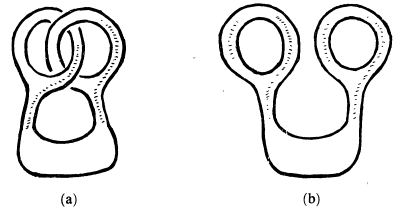
\includegraphics[scale=.6]{enlacement}
\end{center}
\end{quote}
\item Jeffrey Weeks, \emph{The Shape of Space}
\begin{quote}
Également recommandé par Allen Hatcher, pour les mêmes raisons. Rubans de Möbius, bouteilles de Klein, tores, espaces hyperboliques, déformations... Par un \og mathématicien freelance\fg{} suivant les mots de l'auteur, et effectivement un des meilleurs livres pour découvrir ce qu'est réellement la topologie.
\end{quote}
\item Jean-Pierre Petit, \emph{Le Topologicon}
\begin{quote}
La topologie en bande dessinée ! Contient beaucoup de mathématiques ! Librement téléchargeable. 
\end{quote}
\item  Elisabeth Burroni et Jacques Penon, \emph{Topologie ou la géométrie du caoutchouc : 300 exercices corrigés pour le deuxième cycle}
\begin{quote}
Elisabeth Burroni est également l'autrice d'un livre sur la topologie des espaces métriques, accessible au niveau L2/L3.
\end{quote}
\item Colin Adams, \emph{The Knot Book}
\begin{quote}
Ouvrage entièrement dédié à la théorie de noeuds. Mouvements de Reidemeister, graphes, tresses, invariants, polynômes d'Alexander, surfaces bordantes.
\end{quote}
\item André Gramain, \emph{Topologie des surfaces}
\begin{quote}
Cours de L3 à Orsay dans les années 70. L'ouvrage, de seulement 116 pages, s'efforce d'éviter les espaces topologiques généraux afin d'être accessible avec les connaissances des deux premières années, mais il vise des résultats non triviaux de topologie : groupe fondamental, fonctions de Morse, puis classification des surfaces (à l'aide de la théorie de Morse). 
\end{quote}
\item George K. Francis, \emph{A Topological Picturebook}
\end{itemize}


\paragraph{Transition L3-M1 :}
\begin{itemize}

\item L. Christine Kinsey, \emph{Topology of Surfaces}
\begin{quote}
Tiré de la préface : \og cours conçu comme un antidote aux cours allant du général au particulier mais n'atteignant le particulier que lorsque les étudiants sont déjà trop désorientés pour seulement s'y raccrocher.\fg{} Compacts, connexes, continuité, séparation et quotients, surfaces et triangulations, caractéristique d'Euler, homologie, homotopie, topologie différentielle.  276 illustrations.
\end{quote}
\item Jiří Matoušek, \emph{Using the Borsuk-Ulam theorem}
\begin{quote}
Magnifique livre entièrement dédié au théorème de Borsuk-Ulam, sorte de TVI sous stéroïdes, qui permet par exemple d'affirmer qu'à tout moment sur Terre il existe deux points antipodaux ayant même température et même pression. Le livre est écrit avec la collaboration de Anders Björner and Günter Ziegler.
\end{quote}
\item M.A Armstrong, \emph{Basic Topology}
\begin{quote}
Surfaces et théorème d'Euler. Courbes de Peano. Quotients et recollements, ruban de Möbius, groupe fondamental, triangulation, homologie simpliciale, degrés et nombres de Lefschetz, Borsuk-Ulam, revêtements et n\oe uds. 139 illustrations. 
\end{quote}
\item Michael Henle, \emph{A Combinatorial Introduction to Topology}
\begin{quote}
Espaces topologiques, compacité et connexité. champs de vecteurs, lemme de Sperner et théorème de Brouwer, indice de lacets, théorème de Jordan, classification des surfaces. Ensuite, thèmes plus avancés : complexes, homologie, revêtements, point fixe de Lefschetz, homotopie. Très richement illustré, peu de pages sans figures.
\end{quote}
\item Klaus Jänich, \emph{Topology}
\begin{quote}
Grande référence allemande traduite en anglais.  Niveau avancé. \og Concepts fondamentaux\fg{} en dix-huit pages. Bases de voisinages, espaces vectoriels topologiques, topologie quotient, homotopie, CW-complexes. 181 illustrations.
\end{quote}
\item Gustave Choquet, \emph{Cours de topologie}
\begin{quote}
Classique de topologie à la française, porté sur l'analyse. Espaces topologiques, fonctions à valeurs réelles (Stone-Weierstrass), espaces vectoriels topologiques. 334 pages et seulement 6 illustrations.
\end{quote}

\end{itemize}






\section{Autres}


\begin{itemize}
\item John H. Conway, Derek A. Smith \emph{On quaternions and octonions}
\begin{quote}
Avouez, vous \emph{voulez} savoir qu'est-ce que c'est que toutes ces histoires sur les quaternions. Sans doute le meilleur livre d'introduction sur le sujet.
\end{quote}
\item Richard Stanley, \emph{Enumerative Combinatorics, vol. 1}
\begin{quote}
Il fallait bien un livre de combinatoire ou de mathématiques discrètes (en plus du \emph{Mathématiques concrètes}) dans cette liste. Librement téléchargeable sur le site de l'auteur. Les livres de combinatoire pour les olympiades sont également recommandés.
\end{quote}
% mettre aussi Miklos Bona, A Walk Through Combinatorics: An Introduction to Enumeration, Graph Theory, and Selected Other Topics ?
\item Michèle Audin \emph{Souvenirs sur Sofia Kovalevskaya}
\begin{quote}
Biographie de Sofia Kovalevskaya, mathématicienne qui a donné son nom entre autres au théorème de Cauchy-Kowalevskaya (sorte de Cauchy-Lipschitz à plusieurs variables) et qui a eu une vie bien remplie. Personnage vraiment fascinant et lecture passionnante.
\end{quote}
\item Jean Dieudonné, \emph{Abrégé d'histoire des mathématiques}
\begin{quote}
Ouvrage d'histoire des mathématiques, dirigé par Jean Dieudonné, un des fondateurs du groupe Bourbaki et écrit par des mathématiciens. Couvre la période 1700-1900. 
\end{quote}
\item Lynn Arthur Steen et J. Arthur Seebach, Jr., \emph{Counter-examples in topology}
\begin{quote}
Contre-exemples de topologie générale, dépassant le niveau L3. Pour plonger les mains dans le cambouis et avoir conscience des  merveilles (ou horreurs?) se cachant sous le vocable d'\og espace topologique\fg. Attention à ne pas réduire à la topologie à l'étude d'objets ultra-pathologiques. La théorie peut gérer ces objets, mais cela ne constitue pas l'essence de la discipline.
\end{quote}
\item Pierre Bayard \emph{Comment parler des livres que l'on n'a pas lus}
\end{itemize}




\end{document}

A ajouter:

The Art and Craft of Problem Solving de Paul Zeitz

Mathematics: A Very Short Introduction de Timothy Gowers

Mathematics: Its Content, Methods and Meaning de Aleksandrov, Kolmogorov, Lavrent’iev

Letters to a Young Mathematician de Ian Stewart

AUtres livres de Stewart ?



\section{Bibliographie spécifique pour les cours supplémentaires de Magistère}

\subsection{Analyse harmonique et applications à la théorie des nombres}
\begin{itemize}
\item  \emph{}
\begin{quote}

\end{quote}
\item  \emph{}
\begin{quote}

\end{quote}
\item  \emph{}
\begin{quote}

\end{quote}
\end{itemize}

\subsection{Mécanique quantique}
\begin{itemize}
\item L.D. Landau, E. M. Lifshitz, \emph{Mécanique quantique, théorie non relativiste}
\begin{quote}
Troisième tome du Landau-Lifshitz, mythique ouvrage soviétique.
\end{quote}
\item R. Feynman, R. Leighton, M. Sands, \emph{Mécanique quantique}
\begin{quote}
Le tome 5 tome du \og Cours de physique de Feynman\fg. (Feynman, professeur d'université à 24 ans, prix Nobel de physique et grand vulgarisateur.) 
\end{quote}
\item C. Cohen-Tannoudji, \emph{Mécanique quantique}
\begin{quote}
Autre bible de mécanique quantique, cette fois par un prix Nobel made in France.
\end{quote}
\end{itemize}

\subsection{Chaos et systèmes dynamiques}
\begin{itemize}
\item  \emph{}
\begin{quote}

\end{quote}
\item  \emph{}
\begin{quote}

\end{quote}
\item  \emph{}
\begin{quote}

\end{quote}
\end{itemize}

\subsection{Logique et modèles de calcul}
\begin{itemize}
\item  \emph{}
\begin{quote}

\end{quote}
\item  \emph{}
\begin{quote}

\end{quote}
\item  \emph{}
\begin{quote}

\end{quote}
\end{itemize}

\subsection{Analysis Situs : introduction à la topologie algébrique}
\begin{itemize}
\item  \emph{}
\begin{quote}

\end{quote}
\item  \emph{}
\begin{quote}

\end{quote}
\item  \emph{}
\begin{quote}

\end{quote}
\end{itemize}

